\documentclass[a4paper,12pt,oneside]{book}
\usepackage[T1]{fontenc}                                      
\usepackage[utf8]{inputenc}                               
\usepackage[italian]{babel}
\usepackage{amsfonts}
\usepackage{amsthm}
\usepackage{amsmath,amssymb}
\usepackage{array}
\usepackage{arydshln}
\usepackage{braket}
\usepackage{blindtext}
\usepackage{calc}
\usepackage{cancel}
\usepackage{caption}
\usepackage{epsfig}
\usepackage{eucal}
\usepackage{fancyhdr}
\usepackage{geometry}
\usepackage{graphicx}
\usepackage{indentfirst}
\usepackage{hhline}
\usepackage{hyperref}
\hypersetup{
			colorlinks=true,
			linkcolor=black,
			anchorcolor=black,
			citecolor=black,
			urlcolor=black,
			pdftitle={Appunti di Meccanica Quantistica},
			pdfauthor={Vittorio Lubicz}
}

\usepackage{latexsym}
\usepackage{listings} 
\usepackage{longtable}
\usepackage{makeidx}
\usepackage{mathrsfs}
\usepackage{mathdots}
\usepackage{multirow}
\usepackage{nicefrac}
\usepackage{pdfpages}
\usepackage{physics}
\usepackage{setspace}
\usepackage{tikz}
\usepackage{tikz-3dplot}
\usepackage{textcomp}
\usepackage{titlesec,color}
\usepackage{vmargin}
\setpapersize{A4}
\setmarginsrb{35mm}{30mm}{35mm}{30mm}%
             {0mm}{10mm}{0mm}{10mm}



\definecolor{gray75}{gray}{0.75}
\newcommand{\hsp}{\hspace{20pt}}

\titleformat{\chapter}[hang]{\huge\bfseries}{\myfont{\textit{\large{\chaptername\hspace{1pt} \thechapter\hspace{3pt}}}}\textcolor{gray75}{$\mid$}\hspace{0.4cm}}{0pt}{\myfont{\huge\bfseries}}

\titleformat{\section}[hang]{\large\bfseries}{\myfont{\textit{\normalsize{\thesection\hspace{2pt}}}}\hspace{0.4cm}}{0pt}{\myfont{\Huge\bfseries}}

\titleformat{\subsection}[hang]{\large\bfseries}{\myfont{\textit{\small{\thesubsection\hspace{2pt}}}}\hspace{0.4cm}}{0pt}{\myfont{\huge\bfseries}}

\renewcommand{\chaptermark}[1]{\markboth{#1}{}}
\renewcommand{\sectionmark}[1]{\markright{#1}}
\newcommand*{\myfont}{\fontfamily{ppl}\selectfont}

\begin{document}

%*****************LAYOUT PAGINE**************************
\fancypagestyle{plain}{%
\fancyhf{} % cancella tutti i campi di  intestazione e pi\`e di pagina
\fancyfoot[C]{\bfseries \myfont{\thepage}} % tranne il centro
\renewcommand{\headrulewidth}{0pt}
\renewcommand{\footrulewidth}{0pt}}

\fancypagestyle{VS}{
\headheight = 15pt
\lhead[\myfont{\textit{\textbf{\thechapter\nouppercase{\leftmark}}}}]{\myfont{\textit{\textbf{\nouppercase{\leftmark}}}}}
\chead[]{}
\rhead[\myfont{\textbf{\thepage}}]{\myfont{\textbf{\thepage}}}

\lfoot[]{}
\cfoot[]{}
\rfoot[]{}
}
%*******************************************************



\pagestyle{VS}
\setcounter{chapter}{1}
\setcounter{page}{14}
\chapter[Principi fondamentali della M.Q.]{Principi fondamentali\\ della Meccanica \\ Quantistica. Dualismo\\ onda-particella,\\ probabilità ed ampiezze\\ di probabilità, onde ed\\ elettroni\footnote{F1.1-1.8; LL1}}
La \textbf{meccanica quantistica} è la descrizione del comportamento della materia e della luce in tutti i suoi dettagli ed in particolare di ciò che avviene su scala atomica.\\
\textbf{Gli oggetti su scala molto piccola non i comportano come nessuna cosa di cui si possa avere diretta esperienza.} Sotto alcuni aspetti si comportano come onde, sotto altri come particelle, ma in effetti non si comportano come né l'una né l'altra cosa.\\
D'altra parte il \textbf{comportamento quantistico degli oggetti atomici} (elettroni, protoni, neutroni, fotoni e così via) \textbf{è lo stesso per tutti}: sono tutti \textit{onde-particelle}, o qualunque altro nome gli si voglia dare. onde-particelle. \textbf{Una descrizione coerente del comportamento della materia su scala microscopica venne dato, negli anni 1926-1927, principalmente da Schr\"{o}dinger, Heisenberg e Born.}\\
Consideriamo qui le principali caratteristiche di tale descrizione, descrivendo un \textbf{esperimento ideale}, che mette a confronto una particolare situazione sperimentale, il comportamento quantistico degli elettroni con il comportamento d particelle classiche, quali pallottole, ed onde classiche, del tipo di quelle che si formano nell'acqua.
\newpage
\section*{Un esperimento con pallottole}
\begin{figure}[!htbp]
\begin{center}
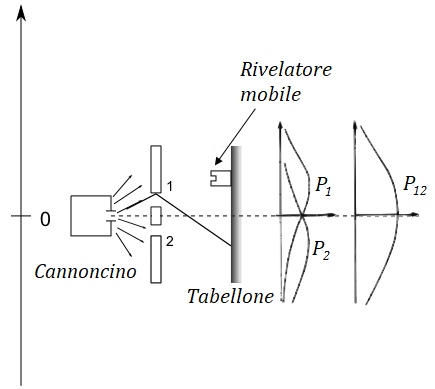
\includegraphics[width=.6\textwidth]{immagini/cap_2/fig_2_1.png}
\end{center}
\end{figure}
\begin{itemize}
\item[\textbf{P$_1=$} ]probabilità che il proiettile giunga in $x$ passando per il foro 1;
\item[\textbf{P$_2=$} ]probabilità che il proiettile giunga in $x$ passando per il foro 2;
\item[\textbf{P$_{12}=$} ]probabilità che il proiettile giunga in $x$ passando per il foro 1 o per il foro 2.
\end{itemize}
\textbf{Risultato dell'esperimento:} I proiettili arrivano sempre a blocchi identici e distinti. L'effetto con entrambi i fori aperti è la somma degli effetti che si hanno quando è aperto ciascuno dei sue fori da solo. Le probabilità vanno sommate:
\begin{equation}
P_{12}=P_1+P_2.
\end{equation}
\textbf{Non si osserva interferenza.}
\newpage
\section*{Un esperimento con onde (prodotte in acqua)}
\begin{figure}[!htbp]
\begin{center}
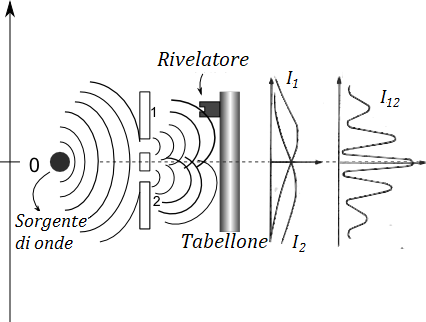
\includegraphics[width=.6\textwidth]{immagini/cap_2/fig_2_2.png}
\end{center}
\end{figure}
\begin{itemize}
\item[\textbf{I$_1=$} ]intensità misurata lasciando aperto solo il foro 1;
\item[\textbf{I$_2=$} ]intensità misurata lasciando aperto solo il foro 2;
\item[\textbf{I$_{12}=$} ]intensità misurata lasciando aperti entrambi i fori.
\end{itemize}
\textbf{Risultato dell'esperimento:} l'intensità  può assumere qualsiasi valore; non possiede una struttura \textit{a blocchi}. \textbf{L'intensità} misurata quando entrambi i fori sono aperti \textbf{non è la somma} di I$_1$ e I$_2$: \textbf{si ha interferenza tra le due onde.}
\subsection*{Matematica dell'interferenza (formalismo complesso)}
\begin{itemize}
\item $\Re{\left(h_1 e^{i\omega t} \right)}=$ altezza istantanea al rivelatore dell'onda proveniente dal foro 1;
\item $\Re{\left(h_2 e^{i\omega t} \right)}=$ altezza istantanea al rivelatore dell'onda proveniente dal foro 2;
\item $\Re{\left( \left(h_1 +h_2 \right) e^{i\omega t} \right)}=$ altezza istantanea al rivelatore dell'onda che arriva quando entrambi i fori sono aperti.
\end{itemize}
L'intensità è proporzionale all'ampiezza quadratica media, cioè, con il famoso formalismo complesso, al modulo quadro dell'ampiezza. Tralasciando la costante di proporzionalità:
\begin{eqnarray}
& &I_1= \lvert {h_1} \rvert ^2, \nonumber \\
& &I_2 \lvert {h_1} \rvert ^2, \\
& &I_{12}= \lvert {h_1+h_2} \rvert ^2= \lvert {h_1} \rvert ^2+ \lvert {h_2} \rvert ^2 + 2 \lvert {h_1} \rvert \lvert {h_2} \rvert \cos \delta ,\nonumber  \\ 
& &\left( \delta = \textrm{ differenza di fase tra } h_1 \textrm{ e } h_2 \textrm{, funzione di }x \right)\nonumber 
\end{eqnarray}
allora, in termini di intensità:
\begin{equation}
I_{12}= I_1 + i_2 + 2 \sqrt{I_1 I_2}\cos \delta.
\end{equation}
L'ultimo termine in questa espressione è il \textbf{termine di interferenza.}
\section*{Un esperimento con elettroni}
\begin{figure}[!htbp]
\begin{center}
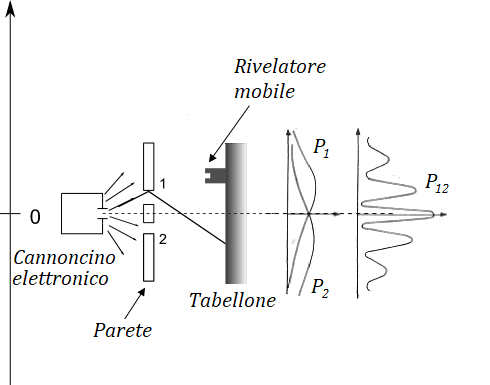
\includegraphics[width=.6\textwidth]{immagini/cap_2/fig_2_3.png}
\end{center}
\end{figure}
\begin{itemize}
\item[\textbf{P$_1=$} ]probabilità che l'elettrone giunga in $x$ passando per il foro 1 (con il foro 2 chiuso);
\item[\textbf{P$_2=$} ]probabilità che l'elettrone giunga in $x$ passando per il foro 2 (con il foro 1 chiuso);
\item[\textbf{P$_{12}=$} ]probabilità che il proiettile giunga in $x$ con entrambi i fori aperti.
\end{itemize}
\textbf{Risultato dell'esperimento:} I proiettili arrivano sempre in granuli, tutti identici tra loro (come i proiettili). La \textbf{probabilità} $P_{12}$ ottenuta con entrambi i fori aperti non è la somma di $P_1$ e $P_2$:
\begin{equation}
P_{12}\neq P_1+P_2.
\end{equation}
Se fosse vero che ciascun elettrone o attraversa il foro 1 oppure attraversa il foro  allora la probabilità $P_{12}$ dovrebbe essere la somma di $P_1$ e $P_2$. Si potrebbe pensare che gli elettroni seguano percorsi complicati, passando magari più volte per ciascun foro. Ma nemmeno questo è possibile:
\begin{itemize}
\item \textbf{vi sono punti n cui} arrivano meno elettroni quando sono aperti entrambi i fori, ossia \textbf{la chiusura di un foro aumenta il numero di elettroni provenienti dall'altro;}
\item \textbf{al centro della curva}, $P_{12}$ è maggiore della somma $P_1 + P_2$,  \textbf{è come se la chiusura di un foro diminuisce il numero di elettroni che escono dall'altro}.
\end{itemize}
Sebbene questi risultati siano incomprensibili, la loro descrizione matematica è estremamente semplice: \textbf{la curva $P_{12}$ è proprio una curva di interferenza come $I_{12}$ e la matematica è dunque quella dell'interferenza.}\\
I risultati dell'esperimento possono essere descritti introducendo due numei complessi, funzione di $\chi$: $\phi _1$ e $\phi _2$. Si ha poi:
\begin{eqnarray}
& P_1= \lvert \phi _1 \rvert ^2, & \\
& P_2= \lvert \phi _2 \rvert ^2, &\\
& P_{12}= \lvert \phi _1 + \phi _2 \rvert ^2. 
\end{eqnarray}
\section*{Osservazione di elettroni}
Poiché il numero di elettroni che arriva in un particolare punto \textbf{non} è uguale al numero di elettroni che arrivano passando dal foro 1 più quelli che passano dal foro 2 ci porta a concludere che \textbf{non è vero che gli elettroni passano attraverso l'uno o l'altro dei fori 1 e 2}. Verifichiamo questa conclusione con un esperimento.\\
Aggiungiamo nell'apparato sperimentale una sorgente di luce, posa dietro allo schermo, a metà tra i due fori. Poiché le cariche elettriche diffondono la luce, quando un elettrone riesce ad attraversare lo schermo devierà verso il nostro occhio della luce e potremo \textit{vedere} il cammino dell'elettrone stesso.
\newpage
\begin{figure}[!htbp]
\begin{center}
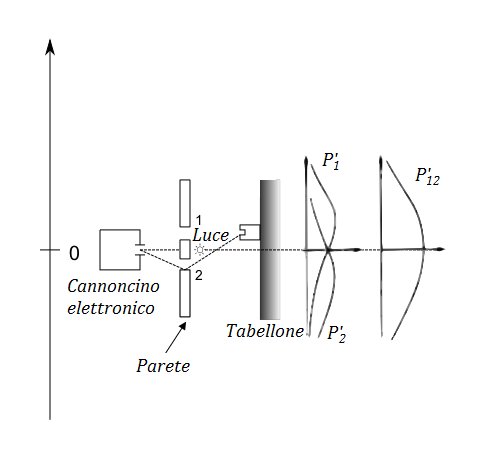
\includegraphics[width=.6\textwidth]{immagini/cap_2/fig_2_4.png}
\end{center}
\end{figure}
\textbf{Risultato dell'esperimento:} Gli elettroni che vengono osservati risultano essere passati o dal foro 1 o dal foro 2 ma non da tutti e due insieme. L'andamento di $P'_1$ e $P'_2$, costruiti lasciando entrambi i fori aperti ma osservando da quale foro sia passato l'elettrone è uguale all'andamento di $P_1$ e $P_2$ osservato nel precedente esperimento chiudendo uno dei due fori. Quindi \textbf{gli elettroni che vediamo arrivare attraverso il foro 1 sono distribuiti nello stesso modo, indipendentemente dalla situazione del foro 2.}\\
La probabilità totale risulta dunque essere la somma delle probabilità
\begin{equation}
P'_{12}= P'_1 + P'_2.
\end{equation}
\textbf{La distribuzione degli elettroni sullo schermo quando li osserviamo è differente da quella quando non li osserviamo}.\\
Evidentemente la luce, nell'essere diffusa dagli elettroni, dà loro un colpo che ne fa mutare il movimento. Si può tentare allora di modificare l'esperimento in modo da osservare gli elettroni senza disturbarli troppo. Ma questo non risulta essere possibile. \textbf{È impossibile costruire un apparecchio per determinare da quale foro è passato l'elettrone che allo stesso tempo non perturbi l'elettrone sufficientemente da distruggere l'interferenza. se un apparecchio è capace di determinare da quale foro è passato l'elettrone  non può essere così delicato da non alterarne in modo essenziale la distribuzione.} Questo risultato è una conseguenza particolare del \textbf{principio di indeterminazione.}
\section[Probabilità e ampiezza di probabilità]{Principi base della Meccanica quantistica: probabilità e ampiezza di probabilità}
Riassumiamo ora, in forma generale le principali conclusioni dell'esperimento sopra descritto:
\begin{enumerate}
\item La probabilità di un evento in un esperimento ideale è data dal quadrato del modulo d un numero complesso $\phi$ che viene detto \textbf{ampiezza di probabilità:}
\begin{eqnarray}
& & P = \textrm{ probabilità}, \nonumber \\
& & \phi = \textrm{ ampiezza di probabilità}, \nonumber \\
& & P = \lvert \phi \rvert ^2 .
\end{eqnarray}
\item Quando un evento può avvenire secondo varie alternative, l'ampiezza di probabilità per l'evento è la somma delle ampiezze di probabilità per le varie alternative considerate separatamente. Si ha perciò interferenza:
\begin{eqnarray}
&\phi = \phi_1 + \phi _2,&  \\
&P = \lvert \phi_1 + \phi _2 \rvert ^2;&
\end{eqnarray}
\item Se si effettua un'esperienza capace di determinare se una o l'altra delle possibili alternative è effettivamente realizzata, la probabilità dell'evento non è la somma delle probabilità per ciascuna delle alternative. Non si ha più interferenza:
\begin{equation}
P= P_1 + P_2.
\end{equation}
\end{enumerate}
Sottolineiamo una differenza molto importante tra la meccanica classica e quella quantistica. \textbf{Nella meccanica quantistica è impossibile prevedere esattamente ciò che accadrà in una data situazione. la sola cosa che è possibile prevedere é la probabilità di eventi differenti.}
\section{Il principio di indeterminazione}
La presenza d interferenza nell'esperimento delle due fenditure, con gli elettroni, mette in risalto come, nel caso di particelle microscopiche, il \textbf{concetto di traiettoria}, che sta a fondamento della meccanica classica, \textbf{viene a perdere di significato nella meccanica quantistica}. Tale circostanza trova la sua espressione nel cosiddetto \textbf{principio di indeterminazione}, uno dei principi basilari della meccanica quantistica, scoperto da \textbf{Heisenberg} nel \textbf{1927}.\\
Se, in seguito ad una misura, ad un elettrone vengono assegnate coordinate determinate, esso non ha, in generale, nessuna velocità determinata. Viceversa se è dotato di una velocità determinata, l'elettrone non potrà avere una posizione determinata nello spazio. Infatti \textbf{l'esistenza simultanea ad ogni istante delle coordinate e delle velocità significherebbe l'esistenza di una traiettoria determinata, che l'elettrone non ha}. Di conseguenza nella meccanica quantistica \textbf{le coordinate e le velocità dell'elettrone sono grandezze che non possono essere misurate con precisione allo stesso istante, cioè non possono avere simultaneamente valori determinati. Si può dire che le coordinate e le velocità dell'elettrone sono grandezze non esistenti simultaneamente.}\\
Una formulazione matematica del principio di indeterminazione è data dalla relazione:
\begin{equation}
\Delta p_x \Delta x \geq \frac{\hbar}{2}.
\end{equation}
\subsection{Il principio di indeterminazione e l'esperimento delle due fenditure}
Mostriamo, in un caso particolare, come il principio di indeterminazione di Heisenberg deve essere valido al fine di evitare situazioni inconsistenti.\\
Immaginiamo di modificare l'esperimento di interferenza degli elettroni sostituendo la parete fissa, con le due fenditure, con una lamina montata su due cuscinetti che si può muovere liberamente in direzione dell'asse x:
\begin{figure}[!htbp]
\begin{center}
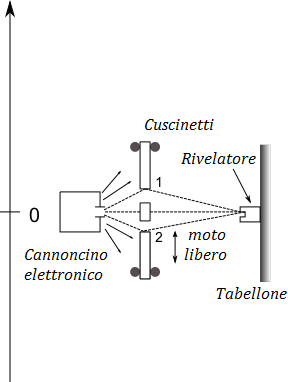
\includegraphics[width=.5\textwidth]{immagini/cap_2/fig_2_5.png}
\end{center}
\end{figure}\\
Osservando il moto della lamina possiamo provare a determinare attraverso quale foro passa un elettrone. Consideriamo infatti il caso in cui il rivelatore è posto in $x=0$. Ci aspettiamo che un elettrone che passi per il foro 1 debba essere deflesso verso il basso dalla lamina per poter arrivare al rivelatore. Poiché la componente verticale dell'impulso dell'elettrone è variata la lamina deve muoversi in direzione opposta con lo stesso impulso. La lamina riceverà quindi una spinta verso l'alto. Se invece l'elettrone passa dal foro inferiore la lamina dovrebbe subire una spinta verso il basso. È chiaro che per ogni posizione del rivelatore l'impulso ricevuto dalla lamina avrà un valore differente a seconda che l'elettrone attraversi il foro 1 o il foro 2. Quindi, \textbf{senza per nulla perturbare gli elettroni, ma solo osservando la lamina, possiamo determinare il percorso scelto dall'elettrone.\\
Tuttavia, per determinare di quanto è variato l'impulso della lamina dopo il passaggio dell'elettrone occorre conoscere l'impulso di questa prima che l'elettrone la attraversi.} Calcoliamo l'impulso che l'elettrone trasmette alla lamina attraversando un foro:\\
\begin{minipage}{.5\textwidth}
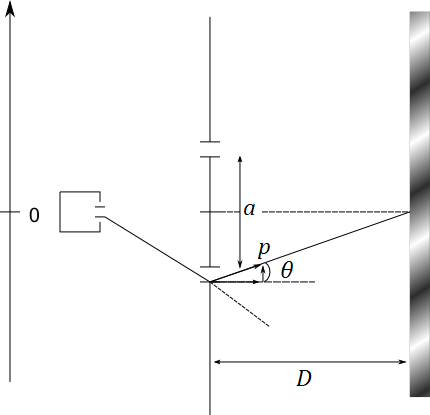
\includegraphics[width=.8\textwidth]{immagini/cap_2/fig_2_6.png}	
\end{minipage}
\hspace{.5cm}
\begin{minipage}{.4\textwidth}
\begin{equation} \tan \theta \simeq \theta \simeq \frac{a}{2D}
\end{equation}
\begin{equation} p_x = p \sin \theta = \frac{pa}{2D}
\end{equation}
\end{minipage}\\
\vspace{.5cm}
l'impulso trovato è dell'ordine di
\begin{equation}
\Delta p \simeq 2p_x = 2p \sin \theta \simeq \frac{pa}{D},
\end{equation}
e questa quantità rappresenta anche l'incertezza massima con la quale è necessario conoscere l'impulso della lacuna prima che l'elettrone l'attraversi per poter distinguere se l'elettrone è passato attraverso il foro 1 o il foro 2.\\
In base al \textbf{principio di indeterminazione}, se l'impulso è noto con una precisione maggiore di $\Delta  p$, allora \textbf{la posizione della lamina stessa non può essere conosciuta con una precisione maggiore di}:
\begin{equation}
\Delta x \simeq \frac{\hbar}{\Delta p} \simeq \frac{\hbar D}{pa}= \frac{\lambda D}{a},
\end{equation}
dove $\lambda = \hbar / p$ è la lunghezza d'onda di De Broglie associata all'elettrone che si muove con impulso $p$.\\
L'incertezza $\Delta x$ allora anche l'incertezza con cui è definita la posizione delle due fenditure, che saranno quindi in diverse posizioni per ogni elettrone che l'attraversi. Questo significa che \textbf{il centro delle frange di interferenza avrà una posizione differente per i vari elettroni.}\\
Dimostreremo ora che la lunghezza $\Delta x$, di cui oscillano lungo l'asse $x$ le frange di interferenza, è circa uguale alla distanza tra due massimi vicini. \textbf{Un tale movimento, che avviene a caso, è giusto sufficiente a distruggere le oscillazioni del grafico e quindi a far s che non si osservi più interferenza.}\\
\vspace{1cm}
\begin{minipage}{.5\textwidth}
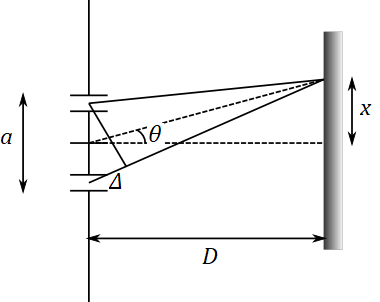
\includegraphics[width=.8\textwidth]{immagini/cap_2/fig_2_7.png}	
\end{minipage}
\begin{minipage}{.5\textwidth}
\begin{equation}
\Delta = a \sin \theta \simeq a \theta = \frac{ax}{D}
\end{equation}
\end{minipage}\\
\vspace{.5cm}
La differenza di fase tra le onde che giungono nel punto $x$ dalle due fenditure è:
\begin{equation}
\delta = k\Delta =\frac{2 \pi }{\lambda}\Delta = \frac{2 \pi a x}{D}.
\end{equation}
I massimi di interferenza si hanno quando la differenza di fase $\delta $ è pari ad un multiplo intero di $2 \pi$, ossia nei punti d coordinate
\begin{equation}
x_n =n\frac{\lambda D}{a}, \qquad n=0,\pm 1, \pm 2, \dots 
\end{equation}
Due massimi consecutivi si trovano dunque a distanza 
\begin{equation}
\Delta x = \frac{\lambda D}{a},
\end{equation}
che coincide con lo spostamento tipico del centro delle frange di interferenza per ciascun elettrone.\\
\textbf{il principio di indeterminazione garantisce quindi che l'aver osservato la fenditura attraverso la quale è passato l'elettrone porta alla scomparsa dell'interferenza.}
\end{document}